\documentclass[twoside]{book}

% Packages required by doxygen
\usepackage{fixltx2e}
\usepackage{calc}
\usepackage{doxygen}
\usepackage[export]{adjustbox} % also loads graphicx
\usepackage{graphicx}
\usepackage[utf8]{inputenc}
\usepackage{makeidx}
\usepackage{multicol}
\usepackage{multirow}
\PassOptionsToPackage{warn}{textcomp}
\usepackage{textcomp}
\usepackage[nointegrals]{wasysym}
\usepackage[table]{xcolor}

% Font selection
\usepackage[T1]{fontenc}
\usepackage[scaled=.90]{helvet}
\usepackage{courier}
\usepackage{amssymb}
\usepackage{sectsty}
\renewcommand{\familydefault}{\sfdefault}
\allsectionsfont{%
  \fontseries{bc}\selectfont%
  \color{darkgray}%
}
\renewcommand{\DoxyLabelFont}{%
  \fontseries{bc}\selectfont%
  \color{darkgray}%
}
\newcommand{\+}{\discretionary{\mbox{\scriptsize$\hookleftarrow$}}{}{}}

% Page & text layout
\usepackage{geometry}
\geometry{%
  a4paper,%
  top=2.5cm,%
  bottom=2.5cm,%
  left=2.5cm,%
  right=2.5cm%
}
\tolerance=750
\hfuzz=15pt
\hbadness=750
\setlength{\emergencystretch}{15pt}
\setlength{\parindent}{0cm}
\setlength{\parskip}{3ex plus 2ex minus 2ex}
\makeatletter
\renewcommand{\paragraph}{%
  \@startsection{paragraph}{4}{0ex}{-1.0ex}{1.0ex}{%
    \normalfont\normalsize\bfseries\SS@parafont%
  }%
}
\renewcommand{\subparagraph}{%
  \@startsection{subparagraph}{5}{0ex}{-1.0ex}{1.0ex}{%
    \normalfont\normalsize\bfseries\SS@subparafont%
  }%
}
\makeatother

% Headers & footers
\usepackage{fancyhdr}
\pagestyle{fancyplain}
\fancyhead[LE]{\fancyplain{}{\bfseries\thepage}}
\fancyhead[CE]{\fancyplain{}{}}
\fancyhead[RE]{\fancyplain{}{\bfseries\leftmark}}
\fancyhead[LO]{\fancyplain{}{\bfseries\rightmark}}
\fancyhead[CO]{\fancyplain{}{}}
\fancyhead[RO]{\fancyplain{}{\bfseries\thepage}}
\fancyfoot[LE]{\fancyplain{}{}}
\fancyfoot[CE]{\fancyplain{}{}}
\fancyfoot[RE]{\fancyplain{}{\bfseries\scriptsize Generated by Doxygen }}
\fancyfoot[LO]{\fancyplain{}{\bfseries\scriptsize Generated by Doxygen }}
\fancyfoot[CO]{\fancyplain{}{}}
\fancyfoot[RO]{\fancyplain{}{}}
\renewcommand{\footrulewidth}{0.4pt}
\renewcommand{\chaptermark}[1]{%
  \markboth{#1}{}%
}
\renewcommand{\sectionmark}[1]{%
  \markright{\thesection\ #1}%
}

% Indices & bibliography
\usepackage{natbib}
\usepackage[titles]{tocloft}
\setcounter{tocdepth}{3}
\setcounter{secnumdepth}{5}
\makeindex

% Hyperlinks (required, but should be loaded last)
\usepackage{ifpdf}
\ifpdf
  \usepackage[pdftex,pagebackref=true]{hyperref}
\else
  \usepackage[ps2pdf,pagebackref=true]{hyperref}
\fi
\hypersetup{%
  colorlinks=true,%
  linkcolor=blue,%
  citecolor=blue,%
  unicode%
}

% Custom commands
\newcommand{\clearemptydoublepage}{%
  \newpage{\pagestyle{empty}\cleardoublepage}%
}

\usepackage{caption}
\captionsetup{labelsep=space,justification=centering,font={bf},singlelinecheck=off,skip=4pt,position=top}

%===== C O N T E N T S =====

\begin{document}

% Titlepage & ToC
\hypersetup{pageanchor=false,
             bookmarksnumbered=true,
             pdfencoding=unicode
            }
\pagenumbering{alph}
\begin{titlepage}
\vspace*{7cm}
\begin{center}%
{\Large Matrix multiplication }\\
\vspace*{1cm}
{\large Generated by Doxygen 1.8.14}\\
\end{center}
\end{titlepage}
\clearemptydoublepage
\pagenumbering{roman}
\tableofcontents
\clearemptydoublepage
\pagenumbering{arabic}
\hypersetup{pageanchor=true}

%--- Begin generated contents ---
\chapter{Namespace Index}
\section{Namespace List}
Here is a list of all documented namespaces with brief descriptions\+:\begin{DoxyCompactList}
\item\contentsline{section}{\mbox{\hyperlink{namespaceMath}{Math}} \\*Classes and definitions related to mathematical objects and operations }{\pageref{namespaceMath}}{}
\item\contentsline{section}{\mbox{\hyperlink{namespaceMatTestUtils}{Mat\+Test\+Utils}} \\*Methods, structures and auxiliar definitions for testing different matrix multiplication approachs }{\pageref{namespaceMatTestUtils}}{}
\end{DoxyCompactList}

\chapter{Hierarchical Index}
\section{Class Hierarchy}
This inheritance list is sorted roughly, but not completely, alphabetically\+:\begin{DoxyCompactList}
\item \contentsline{section}{Matrix$<$ T\+Field $>$}{\pageref{classMatrix}}{}
\item \contentsline{section}{Matrix\+Multiplier$<$ T\+Field $>$}{\pageref{classMatrixMultiplier}}{}
\begin{DoxyCompactList}
\item \contentsline{section}{Concurrent\+Matrix\+Multiplier$<$ T\+Field $>$}{\pageref{classConcurrentMatrixMultiplier}}{}
\item \contentsline{section}{Sequential\+Matrix\+Multiplier$<$ T\+Field $>$}{\pageref{classSequentialMatrixMultiplier}}{}
\end{DoxyCompactList}
\item \contentsline{section}{Mat\+Test\+Utils\+:\+:Perf\+Stats}{\pageref{structMatTestUtils_1_1PerfStats}}{}
\end{DoxyCompactList}

\chapter{Class Index}
\section{Class List}
Here are the classes, structs, unions and interfaces with brief descriptions\+:\begin{DoxyCompactList}
\item\contentsline{section}{\mbox{\hyperlink{classMath_1_1ConcurrentMatrixMultiplier}{Math\+::\+Concurrent\+Matrix\+Multiplier$<$ T\+Field $>$}} \\*Provides a method for multiplying matrices based on the mathematical definition using multiple threads }{\pageref{classMath_1_1ConcurrentMatrixMultiplier}}{}
\item\contentsline{section}{\mbox{\hyperlink{classMath_1_1Matrix}{Math\+::\+Matrix$<$ T\+Field $>$}} \\*Represents an m x n matrix, with its data and some operations }{\pageref{classMath_1_1Matrix}}{}
\item\contentsline{section}{\mbox{\hyperlink{classMath_1_1MatrixMultiplier}{Math\+::\+Matrix\+Multiplier$<$ T\+Field $>$}} \\*Represents an strategy for matrix multiplication }{\pageref{classMath_1_1MatrixMultiplier}}{}
\item\contentsline{section}{\mbox{\hyperlink{structMatTestUtils_1_1PerfStats}{Mat\+Test\+Utils\+::\+Perf\+Stats}} \\*Represent statistical estimators for the running times of the multiplication approaches }{\pageref{structMatTestUtils_1_1PerfStats}}{}
\item\contentsline{section}{\mbox{\hyperlink{classMath_1_1SequentialMatrixMultiplier}{Math\+::\+Sequential\+Matrix\+Multiplier$<$ T\+Field $>$}} \\*Provides a method for multiplying matrices based on the mathematical definition sequentially (single-\/thread) }{\pageref{classMath_1_1SequentialMatrixMultiplier}}{}
\end{DoxyCompactList}

\chapter{Namespace Documentation}
\hypertarget{namespaceMath}{}\section{Math Namespace Reference}
\label{namespaceMath}\index{Math@{Math}}


Classes and definitions related to mathematical objects and operations.  


\subsection*{Classes}
\begin{DoxyCompactItemize}
\item 
class \mbox{\hyperlink{classMath_1_1ConcurrentMatrixMultiplier}{Concurrent\+Matrix\+Multiplier}}
\begin{DoxyCompactList}\small\item\em Provides a method for multiplying matrices based on the mathematical definition using multiple threads. \end{DoxyCompactList}\item 
class \mbox{\hyperlink{classMath_1_1Matrix}{Matrix}}
\begin{DoxyCompactList}\small\item\em Represents an m x n matrix, with its data and some operations. \end{DoxyCompactList}\item 
class \mbox{\hyperlink{classMath_1_1MatrixMultiplier}{Matrix\+Multiplier}}
\begin{DoxyCompactList}\small\item\em Represents an strategy for matrix multiplication. \end{DoxyCompactList}\item 
class \mbox{\hyperlink{classMath_1_1SequentialMatrixMultiplier}{Sequential\+Matrix\+Multiplier}}
\begin{DoxyCompactList}\small\item\em Provides a method for multiplying matrices based on the mathematical definition sequentially (single-\/thread). \end{DoxyCompactList}\end{DoxyCompactItemize}
\subsection*{Functions}
\begin{DoxyCompactItemize}
\item 
{\footnotesize template$<$typename T\+Field $>$ }\\std\+::ostream \& \mbox{\hyperlink{namespaceMath_a03def80e3e35c7171610f7af0390032f}{operator$<$$<$}} (std\+::ostream \&os, const \mbox{\hyperlink{classMath_1_1Matrix}{Math\+::\+Matrix}}$<$ T\+Field $>$ \&matrix)
\begin{DoxyCompactList}\small\item\em Allows printing the matrix by stream. \end{DoxyCompactList}\end{DoxyCompactItemize}


\subsection{Detailed Description}
Classes and definitions related to mathematical objects and operations. 

\subsection{Function Documentation}
\mbox{\Hypertarget{namespaceMath_a03def80e3e35c7171610f7af0390032f}\label{namespaceMath_a03def80e3e35c7171610f7af0390032f}} 
\index{Math@{Math}!operator$<$$<$@{operator$<$$<$}}
\index{operator$<$$<$@{operator$<$$<$}!Math@{Math}}
\subsubsection{\texorpdfstring{operator$<$$<$()}{operator<<()}}
{\footnotesize\ttfamily template$<$typename T\+Field $>$ \\
std\+::ostream \& Math\+::operator$<$$<$ (\begin{DoxyParamCaption}\item[{std\+::ostream \&}]{os,  }\item[{const \mbox{\hyperlink{classMath_1_1Matrix}{Math\+::\+Matrix}}$<$ T\+Field $>$ \&}]{matrix }\end{DoxyParamCaption})}



Allows printing the matrix by stream. 


\begin{DoxyParams}{Parameters}
{\em os} & Output stream. \\
\hline
{\em matrix} & \mbox{\hyperlink{classMath_1_1Matrix}{Matrix}} to be printed. \\
\hline
\end{DoxyParams}

\hypertarget{namespaceMatTestUtils}{}\section{Mat\+Test\+Utils Namespace Reference}
\label{namespaceMatTestUtils}\index{Mat\+Test\+Utils@{Mat\+Test\+Utils}}


Methods, structures and auxiliar definitions for testing different matrix multiplication approachs.  


\subsection*{Classes}
\begin{DoxyCompactItemize}
\item 
struct \mbox{\hyperlink{structMatTestUtils_1_1PerfStats}{Perf\+Stats}}
\begin{DoxyCompactList}\small\item\em Represent statistical estimators for the running times of the multiplication approaches. \end{DoxyCompactList}\end{DoxyCompactItemize}
\subsection*{Enumerations}
\begin{DoxyCompactItemize}
\item 
enum \mbox{\hyperlink{namespaceMatTestUtils_a8ce892071d861e65dd62ef377efaaa6b}{Exec\+Type}} \{ {\bfseries S\+E\+Q\+U\+E\+N\+T\+I\+AL} = 0, 
{\bfseries C\+O\+N\+C\+U\+R\+R\+E\+NT} = 1
 \}
\begin{DoxyCompactList}\small\item\em Types of multipliers. \end{DoxyCompactList}\end{DoxyCompactItemize}
\subsection*{Functions}
\begin{DoxyCompactItemize}
\item 
std\+::ostream \& \mbox{\hyperlink{namespaceMatTestUtils_a8d3fb72c1d83eeaef63f6255186d26c6}{operator$<$$<$}} (std\+::ostream \&os, const \mbox{\hyperlink{structMatTestUtils_1_1PerfStats}{Perf\+Stats}} \&ps)
\begin{DoxyCompactList}\small\item\em Writes the performance statistics using a stream. \end{DoxyCompactList}\item 
void \mbox{\hyperlink{namespaceMatTestUtils_affa961d32d7a7eb7addab0a07767f14f}{read\+\_\+arguments}} (int argc, char const $\ast$argv\mbox{[}$\,$\mbox{]}, int \&n, \mbox{\hyperlink{namespaceMatTestUtils_a8ce892071d861e65dd62ef377efaaa6b}{Exec\+Type}} \&method, bool \&write)
\begin{DoxyCompactList}\small\item\em Read command line arguments as specified in the project requirements. \end{DoxyCompactList}\item 
std\+::string \mbox{\hyperlink{namespaceMatTestUtils_a9e032c504f598952db985df790a0bcaa}{get\+\_\+filename}} (std\+::string matrix\+\_\+name, int n)
\begin{DoxyCompactList}\small\item\em Compose the file name of the test matrices as specified in the project description. \end{DoxyCompactList}\item 
\mbox{\hyperlink{classMath_1_1Matrix}{Math\+::\+Matrix}}$<$ int $>$ \mbox{\hyperlink{namespaceMatTestUtils_afe3ee64f63e541853b625e7ee33f32a8}{read\+\_\+matrix}} (std\+::string filename)
\begin{DoxyCompactList}\small\item\em Read matrix from the a test file, as specified in the project description. \end{DoxyCompactList}\item 
\mbox{\hyperlink{structMatTestUtils_1_1PerfStats}{Perf\+Stats}} \mbox{\hyperlink{namespaceMatTestUtils_acb8180416ec63f236bd49092434ce55e}{mult\+\_\+perf\+\_\+stats}} (const \mbox{\hyperlink{classMath_1_1Matrix}{Math\+::\+Matrix}}$<$ int $>$ \&A, const \mbox{\hyperlink{classMath_1_1Matrix}{Math\+::\+Matrix}}$<$ int $>$ \&B, \mbox{\hyperlink{classMath_1_1Matrix}{Math\+::\+Matrix}}$<$ int $>$ \&C, const int \&nrepeat)
\begin{DoxyCompactList}\small\item\em Multiplies AxB repeated times, returning statistical results about the sequence of the running times. \end{DoxyCompactList}\end{DoxyCompactItemize}
\subsection*{Variables}
\begin{DoxyCompactItemize}
\item 
\mbox{\Hypertarget{namespaceMatTestUtils_ac809b72319e3d38f960650baf31dc1e6}\label{namespaceMatTestUtils_ac809b72319e3d38f960650baf31dc1e6}} 
const int {\bfseries min\+\_\+n} = 4
\item 
\mbox{\Hypertarget{namespaceMatTestUtils_aae57ce6440d799106e6f95f6094b2d6d}\label{namespaceMatTestUtils_aae57ce6440d799106e6f95f6094b2d6d}} 
const int {\bfseries max\+\_\+n} = 2048
\end{DoxyCompactItemize}


\subsection{Detailed Description}
Methods, structures and auxiliar definitions for testing different matrix multiplication approachs. 

This was specifically designed according to the requirements of the proposed work. It has methods for reading matrices from file in a fixed format and testing them, generating statistics about the multiplication performance.

\begin{DoxyAuthor}{Author}
Vitor Greati, Carlos Vieira 
\end{DoxyAuthor}
\begin{DoxyDate}{Date}
2018-\/03-\/25 
\end{DoxyDate}


\subsection{Enumeration Type Documentation}
\mbox{\Hypertarget{namespaceMatTestUtils_a8ce892071d861e65dd62ef377efaaa6b}\label{namespaceMatTestUtils_a8ce892071d861e65dd62ef377efaaa6b}} 
\index{Mat\+Test\+Utils@{Mat\+Test\+Utils}!Exec\+Type@{Exec\+Type}}
\index{Exec\+Type@{Exec\+Type}!Mat\+Test\+Utils@{Mat\+Test\+Utils}}
\subsubsection{\texorpdfstring{Exec\+Type}{ExecType}}
{\footnotesize\ttfamily enum \mbox{\hyperlink{namespaceMatTestUtils_a8ce892071d861e65dd62ef377efaaa6b}{Mat\+Test\+Utils\+::\+Exec\+Type}}}



Types of multipliers. 

Used when it is necessary to check what multiplication approach was requested. 

\subsection{Function Documentation}
\mbox{\Hypertarget{namespaceMatTestUtils_a9e032c504f598952db985df790a0bcaa}\label{namespaceMatTestUtils_a9e032c504f598952db985df790a0bcaa}} 
\index{Mat\+Test\+Utils@{Mat\+Test\+Utils}!get\+\_\+filename@{get\+\_\+filename}}
\index{get\+\_\+filename@{get\+\_\+filename}!Mat\+Test\+Utils@{Mat\+Test\+Utils}}
\subsubsection{\texorpdfstring{get\+\_\+filename()}{get\_filename()}}
{\footnotesize\ttfamily std\+::string Mat\+Test\+Utils\+::get\+\_\+filename (\begin{DoxyParamCaption}\item[{std\+::string}]{matrix\+\_\+name,  }\item[{int}]{n }\end{DoxyParamCaption})}



Compose the file name of the test matrices as specified in the project description. 


\begin{DoxyParams}{Parameters}
{\em matrix\+\_\+name} & Matrix name (A $\vert$ B) \\
\hline
{\em n} & Matrix size. \\
\hline
\end{DoxyParams}
\mbox{\Hypertarget{namespaceMatTestUtils_acb8180416ec63f236bd49092434ce55e}\label{namespaceMatTestUtils_acb8180416ec63f236bd49092434ce55e}} 
\index{Mat\+Test\+Utils@{Mat\+Test\+Utils}!mult\+\_\+perf\+\_\+stats@{mult\+\_\+perf\+\_\+stats}}
\index{mult\+\_\+perf\+\_\+stats@{mult\+\_\+perf\+\_\+stats}!Mat\+Test\+Utils@{Mat\+Test\+Utils}}
\subsubsection{\texorpdfstring{mult\+\_\+perf\+\_\+stats()}{mult\_perf\_stats()}}
{\footnotesize\ttfamily \mbox{\hyperlink{structMatTestUtils_1_1PerfStats}{Perf\+Stats}} Mat\+Test\+Utils\+::mult\+\_\+perf\+\_\+stats (\begin{DoxyParamCaption}\item[{const \mbox{\hyperlink{classMath_1_1Matrix}{Math\+::\+Matrix}}$<$ int $>$ \&}]{A,  }\item[{const \mbox{\hyperlink{classMath_1_1Matrix}{Math\+::\+Matrix}}$<$ int $>$ \&}]{B,  }\item[{\mbox{\hyperlink{classMath_1_1Matrix}{Math\+::\+Matrix}}$<$ int $>$ \&}]{C,  }\item[{const int \&}]{nrepeat }\end{DoxyParamCaption})}



Multiplies AxB repeated times, returning statistical results about the sequence of the running times. 


\begin{DoxyParams}{Parameters}
{\em A} & Left mxn matrix. \\
\hline
{\em B} & Right nxp matrix. \\
\hline
{\em C} & Resulting nxn matrix. \\
\hline
{\em nrepeat} & Number of repetitions. \\
\hline
\end{DoxyParams}
\mbox{\Hypertarget{namespaceMatTestUtils_a8d3fb72c1d83eeaef63f6255186d26c6}\label{namespaceMatTestUtils_a8d3fb72c1d83eeaef63f6255186d26c6}} 
\index{Mat\+Test\+Utils@{Mat\+Test\+Utils}!operator$<$$<$@{operator$<$$<$}}
\index{operator$<$$<$@{operator$<$$<$}!Mat\+Test\+Utils@{Mat\+Test\+Utils}}
\subsubsection{\texorpdfstring{operator$<$$<$()}{operator<<()}}
{\footnotesize\ttfamily std\+::ostream \& Mat\+Test\+Utils\+::operator$<$$<$ (\begin{DoxyParamCaption}\item[{std\+::ostream \&}]{os,  }\item[{const \mbox{\hyperlink{structMatTestUtils_1_1PerfStats}{Perf\+Stats}} \&}]{ps }\end{DoxyParamCaption})}



Writes the performance statistics using a stream. 


\begin{DoxyParams}{Parameters}
{\em os} & Ouput stream. \\
\hline
{\em ps} & Performance statistics. \\
\hline
\end{DoxyParams}
\mbox{\Hypertarget{namespaceMatTestUtils_affa961d32d7a7eb7addab0a07767f14f}\label{namespaceMatTestUtils_affa961d32d7a7eb7addab0a07767f14f}} 
\index{Mat\+Test\+Utils@{Mat\+Test\+Utils}!read\+\_\+arguments@{read\+\_\+arguments}}
\index{read\+\_\+arguments@{read\+\_\+arguments}!Mat\+Test\+Utils@{Mat\+Test\+Utils}}
\subsubsection{\texorpdfstring{read\+\_\+arguments()}{read\_arguments()}}
{\footnotesize\ttfamily void Mat\+Test\+Utils\+::read\+\_\+arguments (\begin{DoxyParamCaption}\item[{int}]{argc,  }\item[{char const $\ast$}]{argv\mbox{[}$\,$\mbox{]},  }\item[{int \&}]{n,  }\item[{\mbox{\hyperlink{namespaceMatTestUtils_a8ce892071d861e65dd62ef377efaaa6b}{Exec\+Type}} \&}]{method,  }\item[{bool \&}]{write }\end{DoxyParamCaption})}



Read command line arguments as specified in the project requirements. 


\begin{DoxyParams}{Parameters}
{\em argc} & Number of arguments. \\
\hline
{\em argv} & Arguments. \\
\hline
{\em n} & Matrix size. \\
\hline
{\em method} & Required method. \\
\hline
{\em write} & True if the result matrix must be written in a file. \\
\hline
\end{DoxyParams}
\mbox{\Hypertarget{namespaceMatTestUtils_afe3ee64f63e541853b625e7ee33f32a8}\label{namespaceMatTestUtils_afe3ee64f63e541853b625e7ee33f32a8}} 
\index{Mat\+Test\+Utils@{Mat\+Test\+Utils}!read\+\_\+matrix@{read\+\_\+matrix}}
\index{read\+\_\+matrix@{read\+\_\+matrix}!Mat\+Test\+Utils@{Mat\+Test\+Utils}}
\subsubsection{\texorpdfstring{read\+\_\+matrix()}{read\_matrix()}}
{\footnotesize\ttfamily \mbox{\hyperlink{classMath_1_1Matrix}{Math\+::\+Matrix}}$<$ int $>$ Mat\+Test\+Utils\+::read\+\_\+matrix (\begin{DoxyParamCaption}\item[{std\+::string}]{filename }\end{DoxyParamCaption})}



Read matrix from the a test file, as specified in the project description. 


\begin{DoxyParams}{Parameters}
{\em filename} & Filename. \\
\hline
\end{DoxyParams}

\chapter{Class Documentation}
\hypertarget{classMath_1_1ConcurrentMatrixMultiplier}{}\section{Math\+:\+:Concurrent\+Matrix\+Multiplier$<$ T\+Field $>$ Class Template Reference}
\label{classMath_1_1ConcurrentMatrixMultiplier}\index{Math\+::\+Concurrent\+Matrix\+Multiplier$<$ T\+Field $>$@{Math\+::\+Concurrent\+Matrix\+Multiplier$<$ T\+Field $>$}}


Provides a method for multiplying matrices based on the mathematical definition using multiple threads.  




{\ttfamily \#include $<$Concurrent\+Matrix\+Multiplier.\+h$>$}

Inheritance diagram for Math\+:\+:Concurrent\+Matrix\+Multiplier$<$ T\+Field $>$\+:\begin{figure}[H]
\begin{center}
\leavevmode
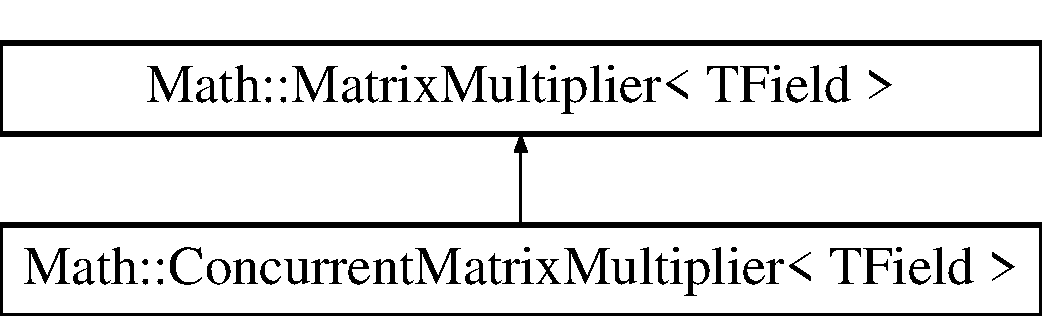
\includegraphics[height=2.000000cm]{classMath_1_1ConcurrentMatrixMultiplier}
\end{center}
\end{figure}
\subsection*{Public Member Functions}
\begin{DoxyCompactItemize}
\item 
void \mbox{\hyperlink{classMath_1_1ConcurrentMatrixMultiplier_aff05c55c52bf7b9fb58b5a52d5247e7d}{multiply}} (const \mbox{\hyperlink{classMath_1_1Matrix}{Matrix}}$<$ T\+Field $>$ \&A, const \mbox{\hyperlink{classMath_1_1Matrix}{Matrix}}$<$ T\+Field $>$ \&B, \mbox{\hyperlink{classMath_1_1Matrix}{Matrix}}$<$ T\+Field $>$ \&C)
\begin{DoxyCompactList}\small\item\em Computes the product of two matrices using the algorithm from the mathematical definition, using multiple threads. \end{DoxyCompactList}\item 
void \mbox{\hyperlink{classMath_1_1ConcurrentMatrixMultiplier_ac6ab99958d957a7461819455a2114483}{compute\+\_\+mult\+\_\+line}} (const \mbox{\hyperlink{classMath_1_1Matrix}{Matrix}}$<$ T\+Field $>$ \&A, const \mbox{\hyperlink{classMath_1_1Matrix}{Matrix}}$<$ T\+Field $>$ \&B, \mbox{\hyperlink{classMath_1_1Matrix}{Matrix}}$<$ T\+Field $>$ \&C, const int \&i)
\begin{DoxyCompactList}\small\item\em Basic operation for computing one row of the product matrix. \end{DoxyCompactList}\end{DoxyCompactItemize}


\subsection{Detailed Description}
\subsubsection*{template$<$typename T\+Field$>$\newline
class Math\+::\+Concurrent\+Matrix\+Multiplier$<$ T\+Field $>$}

Provides a method for multiplying matrices based on the mathematical definition using multiple threads. 

\begin{DoxyAuthor}{Author}
Vitor Greati, Carlos Vieira 
\end{DoxyAuthor}
\begin{DoxyDate}{Date}
2018-\/03-\/28 
\end{DoxyDate}


\subsection{Member Function Documentation}
\mbox{\Hypertarget{classMath_1_1ConcurrentMatrixMultiplier_ac6ab99958d957a7461819455a2114483}\label{classMath_1_1ConcurrentMatrixMultiplier_ac6ab99958d957a7461819455a2114483}} 
\index{Math\+::\+Concurrent\+Matrix\+Multiplier@{Math\+::\+Concurrent\+Matrix\+Multiplier}!compute\+\_\+mult\+\_\+line@{compute\+\_\+mult\+\_\+line}}
\index{compute\+\_\+mult\+\_\+line@{compute\+\_\+mult\+\_\+line}!Math\+::\+Concurrent\+Matrix\+Multiplier@{Math\+::\+Concurrent\+Matrix\+Multiplier}}
\subsubsection{\texorpdfstring{compute\+\_\+mult\+\_\+line()}{compute\_mult\_line()}}
{\footnotesize\ttfamily template$<$typename T\+Field $>$ \\
void \mbox{\hyperlink{classMath_1_1ConcurrentMatrixMultiplier}{Math\+::\+Concurrent\+Matrix\+Multiplier}}$<$ T\+Field $>$\+::compute\+\_\+mult\+\_\+line (\begin{DoxyParamCaption}\item[{const \mbox{\hyperlink{classMath_1_1Matrix}{Matrix}}$<$ T\+Field $>$ \&}]{A,  }\item[{const \mbox{\hyperlink{classMath_1_1Matrix}{Matrix}}$<$ T\+Field $>$ \&}]{B,  }\item[{\mbox{\hyperlink{classMath_1_1Matrix}{Matrix}}$<$ T\+Field $>$ \&}]{C,  }\item[{const int \&}]{i }\end{DoxyParamCaption})\hspace{0.3cm}{\ttfamily [inline]}}



Basic operation for computing one row of the product matrix. 


\begin{DoxyParams}{Parameters}
{\em A} & Left operand. \\
\hline
{\em B} & Right operand. \\
\hline
{\em C} & Product matrix. \\
\hline
{\em i} & Row index of the product matrix. \\
\hline
\end{DoxyParams}
\mbox{\Hypertarget{classMath_1_1ConcurrentMatrixMultiplier_aff05c55c52bf7b9fb58b5a52d5247e7d}\label{classMath_1_1ConcurrentMatrixMultiplier_aff05c55c52bf7b9fb58b5a52d5247e7d}} 
\index{Math\+::\+Concurrent\+Matrix\+Multiplier@{Math\+::\+Concurrent\+Matrix\+Multiplier}!multiply@{multiply}}
\index{multiply@{multiply}!Math\+::\+Concurrent\+Matrix\+Multiplier@{Math\+::\+Concurrent\+Matrix\+Multiplier}}
\subsubsection{\texorpdfstring{multiply()}{multiply()}}
{\footnotesize\ttfamily template$<$typename T\+Field $>$ \\
void \mbox{\hyperlink{classMath_1_1ConcurrentMatrixMultiplier}{Math\+::\+Concurrent\+Matrix\+Multiplier}}$<$ T\+Field $>$\+::multiply (\begin{DoxyParamCaption}\item[{const \mbox{\hyperlink{classMath_1_1Matrix}{Matrix}}$<$ T\+Field $>$ \&}]{A,  }\item[{const \mbox{\hyperlink{classMath_1_1Matrix}{Matrix}}$<$ T\+Field $>$ \&}]{B,  }\item[{\mbox{\hyperlink{classMath_1_1Matrix}{Matrix}}$<$ T\+Field $>$ \&}]{C }\end{DoxyParamCaption})\hspace{0.3cm}{\ttfamily [inline]}, {\ttfamily [virtual]}}



Computes the product of two matrices using the algorithm from the mathematical definition, using multiple threads. 

Allocates one thread for each product row computation. Must be used with caution, since big matrices may surpass some operation system limits when dealing with threads.


\begin{DoxyParams}{Parameters}
{\em A} & Left operand. \\
\hline
{\em B} & Right operand. \\
\hline
{\em C} & Product matrix. \\
\hline
\end{DoxyParams}


Implements \mbox{\hyperlink{classMath_1_1MatrixMultiplier}{Math\+::\+Matrix\+Multiplier$<$ T\+Field $>$}}.



The documentation for this class was generated from the following file\+:\begin{DoxyCompactItemize}
\item 
include/Concurrent\+Matrix\+Multiplier.\+h\end{DoxyCompactItemize}

\hypertarget{classMath_1_1Matrix}{}\section{Math\+:\+:Matrix$<$ T\+Field $>$ Class Template Reference}
\label{classMath_1_1Matrix}\index{Math\+::\+Matrix$<$ T\+Field $>$@{Math\+::\+Matrix$<$ T\+Field $>$}}


Represents an m x n matrix, with its data and some operations.  




{\ttfamily \#include $<$Matrix.\+h$>$}

\subsection*{Public Member Functions}
\begin{DoxyCompactItemize}
\item 
\mbox{\hyperlink{classMath_1_1Matrix_a15145cfc26ef1fd2f68e4a4489490e30}{Matrix}} (const int \&\+\_\+m, const int \&\+\_\+n, const T\+Field \&\+\_\+diag, const T\+Field \&\+\_\+others)
\begin{DoxyCompactList}\small\item\em Constructor for an m x n matrix, accepting values for diagonal elements and others. \end{DoxyCompactList}\item 
\mbox{\hyperlink{classMath_1_1Matrix_ae0d9fbd3225b9b3d50f7b42de14cead6}{Matrix}} (const int \&\+\_\+m, const int \&\+\_\+n, const T\+Field \&\+\_\+initial)
\begin{DoxyCompactList}\small\item\em Constructor for an m x n matrix, with an initial elements. \end{DoxyCompactList}\item 
\mbox{\hyperlink{classMath_1_1Matrix_a3e7c39f3d5951f365f687341cfb0feef}{Matrix}} (const std\+::initializer\+\_\+list$<$ std\+::initializer\+\_\+list$<$ T\+Field $>$$>$ \&l)
\begin{DoxyCompactList}\small\item\em Constructor which takes an initializer list. \end{DoxyCompactList}\item 
\mbox{\hyperlink{classMath_1_1Matrix_a2b849f680fc4ba0d5b0277f1b3116b81}{Matrix}} (const int \&n, const T\+Field $\ast$array)
\begin{DoxyCompactList}\small\item\em Constructor for a one dimensional matrix from a native array. \end{DoxyCompactList}\item 
\mbox{\Hypertarget{classMath_1_1Matrix_adc2c049cc6c6341c4088c6ec6e6fd084}\label{classMath_1_1Matrix_adc2c049cc6c6341c4088c6ec6e6fd084}} 
\mbox{\hyperlink{classMath_1_1Matrix_adc2c049cc6c6341c4088c6ec6e6fd084}{Matrix}} (const \mbox{\hyperlink{classMath_1_1Matrix}{Matrix}}$<$ T\+Field $>$ \&from)
\begin{DoxyCompactList}\small\item\em Copy constructor. \end{DoxyCompactList}\item 
\mbox{\Hypertarget{classMath_1_1Matrix_aacd788cf0658928929d9c381f95cd060}\label{classMath_1_1Matrix_aacd788cf0658928929d9c381f95cd060}} 
\mbox{\hyperlink{classMath_1_1Matrix_aacd788cf0658928929d9c381f95cd060}{$\sim$\+Matrix}} ()
\begin{DoxyCompactList}\small\item\em Destructor for deleting the matrix data. \end{DoxyCompactList}\item 
const T\+Field \& \mbox{\hyperlink{classMath_1_1Matrix_a41b0dc600e73ce6efaea25e0d8501496}{at}} (const int \&i, const int \&j) const
\begin{DoxyCompactList}\small\item\em Access function\+: takes the element data\mbox{[}i\mbox{]}\mbox{[}j\mbox{]}. \end{DoxyCompactList}\item 
void \mbox{\hyperlink{classMath_1_1Matrix_aa45b37d9f91280cee76233e37975046b}{set}} (const int \&i, const int \&j, const T\+Field \&value)
\begin{DoxyCompactList}\small\item\em Set function\+: set data\mbox{[}i\mbox{]}\mbox{[}j\mbox{]} to a value. \end{DoxyCompactList}\item 
T\+Field $\ast$\& \mbox{\hyperlink{classMath_1_1Matrix_ac2ab22aff5aaa615f58fb42a64e1e698}{operator\mbox{[}$\,$\mbox{]}}} (const int \&i)
\begin{DoxyCompactList}\small\item\em Operator \mbox{[}\mbox{]} for accessing rows of a matrix. \end{DoxyCompactList}\item 
T\+Field $\ast$ \mbox{\hyperlink{classMath_1_1Matrix_af7be31f5a4a0448fe4b4f6c9d3893879}{operator\mbox{[}$\,$\mbox{]}}} (const int \&i) const
\begin{DoxyCompactList}\small\item\em Operator \mbox{[}\mbox{]} for accessing rows of a matrix; this returns a copy. \end{DoxyCompactList}\item 
\mbox{\hyperlink{classMath_1_1Matrix}{Matrix}}$<$ T\+Field $>$ \mbox{\hyperlink{classMath_1_1Matrix_a0a501679a182d8556083fcba2245a50f}{operator$\ast$}} (const \mbox{\hyperlink{classMath_1_1Matrix}{Matrix}}$<$ T\+Field $>$ \&\+\_\+rhs) const
\begin{DoxyCompactList}\small\item\em Operator for multiplication of matrices. \end{DoxyCompactList}\item 
void \mbox{\hyperlink{classMath_1_1Matrix_a09f512babb6fb371f3b3978e89e4a05b}{set\+\_\+multiplier}} (\mbox{\hyperlink{classMath_1_1MatrixMultiplier}{Matrix\+Multiplier}}$<$ T\+Field $>$ $\ast$multiplier)
\begin{DoxyCompactList}\small\item\em Set the strategy for multiplication. \end{DoxyCompactList}\item 
\mbox{\hyperlink{classMath_1_1Matrix}{Matrix}}$<$ T\+Field $>$ \& \mbox{\hyperlink{classMath_1_1Matrix_a74a286ee8e6acb9bb1bc6c2b77c0708b}{operator=}} (\mbox{\hyperlink{classMath_1_1Matrix}{Matrix}}$<$ T\+Field $>$ m)
\begin{DoxyCompactList}\small\item\em Operator for assignment. \end{DoxyCompactList}\end{DoxyCompactItemize}
\subsection*{Public Attributes}
\begin{DoxyCompactItemize}
\item 
int \mbox{\hyperlink{classMath_1_1Matrix_a5c1383f7befaac0c43660f75614c8bd5}{rows}}
\item 
int \mbox{\hyperlink{classMath_1_1Matrix_ad9f2871b3b80b076d000f5f95c8ca8c5}{cols}}
\end{DoxyCompactItemize}


\subsection{Detailed Description}
\subsubsection*{template$<$typename T\+Field$>$\newline
class Math\+::\+Matrix$<$ T\+Field $>$}

Represents an m x n matrix, with its data and some operations. 

It is, actually, a template class, which receives, as template argument, the field of the vector space to which the represented matrix belongs. This is a simplified matrix class, which presents only the multiplication operation (through an Strategy) and some auxiliar methods, such as matrix assignment and element access and modification.

\begin{DoxyAuthor}{Author}
Vitor Greati, Carlos Vieira 
\end{DoxyAuthor}
\begin{DoxyDate}{Date}
2018-\/04-\/29 
\end{DoxyDate}
\begin{DoxyVersion}{Version}
1.\+0 
\end{DoxyVersion}


\subsection{Constructor \& Destructor Documentation}
\mbox{\Hypertarget{classMath_1_1Matrix_a15145cfc26ef1fd2f68e4a4489490e30}\label{classMath_1_1Matrix_a15145cfc26ef1fd2f68e4a4489490e30}} 
\index{Math\+::\+Matrix@{Math\+::\+Matrix}!Matrix@{Matrix}}
\index{Matrix@{Matrix}!Math\+::\+Matrix@{Math\+::\+Matrix}}
\subsubsection{\texorpdfstring{Matrix()}{Matrix()}\hspace{0.1cm}{\footnotesize\ttfamily [1/4]}}
{\footnotesize\ttfamily template$<$typename T\+Field $>$ \\
\mbox{\hyperlink{classMath_1_1Matrix}{Math\+::\+Matrix}}$<$ T\+Field $>$\+::\mbox{\hyperlink{classMath_1_1Matrix}{Matrix}} (\begin{DoxyParamCaption}\item[{const int \&}]{\+\_\+m,  }\item[{const int \&}]{\+\_\+n,  }\item[{const T\+Field \&}]{\+\_\+diag,  }\item[{const T\+Field \&}]{\+\_\+others }\end{DoxyParamCaption})}



Constructor for an m x n matrix, accepting values for diagonal elements and others. 

It accepts two values\+: \+\_\+diag, which is the value for filling the diagonal; and \+\_\+others, which fills the other matrix positions.


\begin{DoxyParams}{Parameters}
{\em \+\_\+m} & Number of lines. \\
\hline
{\em \+\_\+n} & Number of columns. \\
\hline
{\em \+\_\+diag} & Initial value for cells in the diagonal. \\
\hline
{\em \+\_\+others} & Initial value for the other cells. \\
\hline
\end{DoxyParams}
\mbox{\Hypertarget{classMath_1_1Matrix_ae0d9fbd3225b9b3d50f7b42de14cead6}\label{classMath_1_1Matrix_ae0d9fbd3225b9b3d50f7b42de14cead6}} 
\index{Math\+::\+Matrix@{Math\+::\+Matrix}!Matrix@{Matrix}}
\index{Matrix@{Matrix}!Math\+::\+Matrix@{Math\+::\+Matrix}}
\subsubsection{\texorpdfstring{Matrix()}{Matrix()}\hspace{0.1cm}{\footnotesize\ttfamily [2/4]}}
{\footnotesize\ttfamily template$<$typename T\+Field $>$ \\
\mbox{\hyperlink{classMath_1_1Matrix}{Math\+::\+Matrix}}$<$ T\+Field $>$\+::\mbox{\hyperlink{classMath_1_1Matrix}{Matrix}} (\begin{DoxyParamCaption}\item[{const int \&}]{\+\_\+m,  }\item[{const int \&}]{\+\_\+n,  }\item[{const T\+Field \&}]{\+\_\+initial }\end{DoxyParamCaption})}



Constructor for an m x n matrix, with an initial elements. 


\begin{DoxyParams}{Parameters}
{\em \+\_\+m} & Number of lines and columns. \\
\hline
{\em \+\_\+initial} & Fill the matrix with this element. \\
\hline
\end{DoxyParams}
\mbox{\Hypertarget{classMath_1_1Matrix_a3e7c39f3d5951f365f687341cfb0feef}\label{classMath_1_1Matrix_a3e7c39f3d5951f365f687341cfb0feef}} 
\index{Math\+::\+Matrix@{Math\+::\+Matrix}!Matrix@{Matrix}}
\index{Matrix@{Matrix}!Math\+::\+Matrix@{Math\+::\+Matrix}}
\subsubsection{\texorpdfstring{Matrix()}{Matrix()}\hspace{0.1cm}{\footnotesize\ttfamily [3/4]}}
{\footnotesize\ttfamily template$<$typename T\+Field $>$ \\
\mbox{\hyperlink{classMath_1_1Matrix}{Math\+::\+Matrix}}$<$ T\+Field $>$\+::\mbox{\hyperlink{classMath_1_1Matrix}{Matrix}} (\begin{DoxyParamCaption}\item[{const std\+::initializer\+\_\+list$<$ std\+::initializer\+\_\+list$<$ T\+Field $>$$>$ \&}]{l }\end{DoxyParamCaption})}



Constructor which takes an initializer list. 


\begin{DoxyParams}{Parameters}
{\em l} & Initializer list with matrix elements. \\
\hline
\end{DoxyParams}
\mbox{\Hypertarget{classMath_1_1Matrix_a2b849f680fc4ba0d5b0277f1b3116b81}\label{classMath_1_1Matrix_a2b849f680fc4ba0d5b0277f1b3116b81}} 
\index{Math\+::\+Matrix@{Math\+::\+Matrix}!Matrix@{Matrix}}
\index{Matrix@{Matrix}!Math\+::\+Matrix@{Math\+::\+Matrix}}
\subsubsection{\texorpdfstring{Matrix()}{Matrix()}\hspace{0.1cm}{\footnotesize\ttfamily [4/4]}}
{\footnotesize\ttfamily template$<$typename T\+Field $>$ \\
\mbox{\hyperlink{classMath_1_1Matrix}{Math\+::\+Matrix}}$<$ T\+Field $>$\+::\mbox{\hyperlink{classMath_1_1Matrix}{Matrix}} (\begin{DoxyParamCaption}\item[{const int \&}]{n,  }\item[{const T\+Field $\ast$}]{array }\end{DoxyParamCaption})}



Constructor for a one dimensional matrix from a native array. 


\begin{DoxyParams}{Parameters}
{\em l} & Array with elements of the vector. \\
\hline
\end{DoxyParams}


\subsection{Member Function Documentation}
\mbox{\Hypertarget{classMath_1_1Matrix_a41b0dc600e73ce6efaea25e0d8501496}\label{classMath_1_1Matrix_a41b0dc600e73ce6efaea25e0d8501496}} 
\index{Math\+::\+Matrix@{Math\+::\+Matrix}!at@{at}}
\index{at@{at}!Math\+::\+Matrix@{Math\+::\+Matrix}}
\subsubsection{\texorpdfstring{at()}{at()}}
{\footnotesize\ttfamily template$<$typename T\+Field $>$ \\
const T\+Field \& \mbox{\hyperlink{classMath_1_1Matrix}{Math\+::\+Matrix}}$<$ T\+Field $>$\+::at (\begin{DoxyParamCaption}\item[{const int \&}]{i,  }\item[{const int \&}]{j }\end{DoxyParamCaption}) const}



Access function\+: takes the element data\mbox{[}i\mbox{]}\mbox{[}j\mbox{]}. 


\begin{DoxyParams}{Parameters}
{\em i} & Element row. \\
\hline
{\em j} & Element column. \\
\hline
\end{DoxyParams}
\mbox{\Hypertarget{classMath_1_1Matrix_a0a501679a182d8556083fcba2245a50f}\label{classMath_1_1Matrix_a0a501679a182d8556083fcba2245a50f}} 
\index{Math\+::\+Matrix@{Math\+::\+Matrix}!operator$\ast$@{operator$\ast$}}
\index{operator$\ast$@{operator$\ast$}!Math\+::\+Matrix@{Math\+::\+Matrix}}
\subsubsection{\texorpdfstring{operator$\ast$()}{operator*()}}
{\footnotesize\ttfamily template$<$typename T\+Field $>$ \\
\mbox{\hyperlink{classMath_1_1Matrix}{Math\+::\+Matrix}}$<$ T\+Field $>$ \mbox{\hyperlink{classMath_1_1Matrix}{Math\+::\+Matrix}}$<$ T\+Field $>$\+::operator$\ast$ (\begin{DoxyParamCaption}\item[{const \mbox{\hyperlink{classMath_1_1Matrix}{Matrix}}$<$ T\+Field $>$ \&}]{\+\_\+rhs }\end{DoxyParamCaption}) const}



Operator for multiplication of matrices. 


\begin{DoxyParams}{Parameters}
{\em \+\_\+rhs} & The matrix to right-\/multiply this matrix. \\
\hline
\end{DoxyParams}
\mbox{\Hypertarget{classMath_1_1Matrix_a74a286ee8e6acb9bb1bc6c2b77c0708b}\label{classMath_1_1Matrix_a74a286ee8e6acb9bb1bc6c2b77c0708b}} 
\index{Math\+::\+Matrix@{Math\+::\+Matrix}!operator=@{operator=}}
\index{operator=@{operator=}!Math\+::\+Matrix@{Math\+::\+Matrix}}
\subsubsection{\texorpdfstring{operator=()}{operator=()}}
{\footnotesize\ttfamily template$<$typename T\+Field $>$ \\
\mbox{\hyperlink{classMath_1_1Matrix}{Math\+::\+Matrix}}$<$ T\+Field $>$ \& \mbox{\hyperlink{classMath_1_1Matrix}{Math\+::\+Matrix}}$<$ T\+Field $>$\+::operator= (\begin{DoxyParamCaption}\item[{\mbox{\hyperlink{classMath_1_1Matrix}{Matrix}}$<$ T\+Field $>$}]{m }\end{DoxyParamCaption})}



Operator for assignment. 


\begin{DoxyParams}{Parameters}
{\em m} & The current object will be equal to m. \\
\hline
\end{DoxyParams}
\mbox{\Hypertarget{classMath_1_1Matrix_ac2ab22aff5aaa615f58fb42a64e1e698}\label{classMath_1_1Matrix_ac2ab22aff5aaa615f58fb42a64e1e698}} 
\index{Math\+::\+Matrix@{Math\+::\+Matrix}!operator\mbox{[}\mbox{]}@{operator[]}}
\index{operator\mbox{[}\mbox{]}@{operator[]}!Math\+::\+Matrix@{Math\+::\+Matrix}}
\subsubsection{\texorpdfstring{operator[]()}{operator[]()}\hspace{0.1cm}{\footnotesize\ttfamily [1/2]}}
{\footnotesize\ttfamily template$<$typename T\+Field $>$ \\
T\+Field $\ast$\& \mbox{\hyperlink{classMath_1_1Matrix}{Math\+::\+Matrix}}$<$ T\+Field $>$\+::operator\mbox{[}$\,$\mbox{]} (\begin{DoxyParamCaption}\item[{const int \&}]{i }\end{DoxyParamCaption})}



Operator \mbox{[}\mbox{]} for accessing rows of a matrix. 

This returns a reference.

Since arrays have \mbox{[}\mbox{]} access defined, this overload allows using \mbox{[}\mbox{]}\mbox{[}\mbox{]} for accessing and modifying matrix elements.


\begin{DoxyParams}{Parameters}
{\em j} & Row index. \\
\hline
\end{DoxyParams}
\begin{DoxyReturn}{Returns}
Pointer to the first element of the row. 
\end{DoxyReturn}
\mbox{\Hypertarget{classMath_1_1Matrix_af7be31f5a4a0448fe4b4f6c9d3893879}\label{classMath_1_1Matrix_af7be31f5a4a0448fe4b4f6c9d3893879}} 
\index{Math\+::\+Matrix@{Math\+::\+Matrix}!operator\mbox{[}\mbox{]}@{operator[]}}
\index{operator\mbox{[}\mbox{]}@{operator[]}!Math\+::\+Matrix@{Math\+::\+Matrix}}
\subsubsection{\texorpdfstring{operator[]()}{operator[]()}\hspace{0.1cm}{\footnotesize\ttfamily [2/2]}}
{\footnotesize\ttfamily template$<$typename T\+Field $>$ \\
T\+Field $\ast$ \mbox{\hyperlink{classMath_1_1Matrix}{Math\+::\+Matrix}}$<$ T\+Field $>$\+::operator\mbox{[}$\,$\mbox{]} (\begin{DoxyParamCaption}\item[{const int \&}]{i }\end{DoxyParamCaption}) const}



Operator \mbox{[}\mbox{]} for accessing rows of a matrix; this returns a copy. 

Since arrays have \mbox{[}\mbox{]} access defined, this overload allows using \mbox{[}\mbox{]}\mbox{[}\mbox{]} for accessing matrix elements.


\begin{DoxyParams}{Parameters}
{\em j} & Row index. \\
\hline
\end{DoxyParams}
\begin{DoxyReturn}{Returns}
Pointer to the first element of the row. 
\end{DoxyReturn}
\mbox{\Hypertarget{classMath_1_1Matrix_aa45b37d9f91280cee76233e37975046b}\label{classMath_1_1Matrix_aa45b37d9f91280cee76233e37975046b}} 
\index{Math\+::\+Matrix@{Math\+::\+Matrix}!set@{set}}
\index{set@{set}!Math\+::\+Matrix@{Math\+::\+Matrix}}
\subsubsection{\texorpdfstring{set()}{set()}}
{\footnotesize\ttfamily template$<$typename T\+Field $>$ \\
void \mbox{\hyperlink{classMath_1_1Matrix}{Math\+::\+Matrix}}$<$ T\+Field $>$\+::set (\begin{DoxyParamCaption}\item[{const int \&}]{i,  }\item[{const int \&}]{j,  }\item[{const T\+Field \&}]{value }\end{DoxyParamCaption})}



Set function\+: set data\mbox{[}i\mbox{]}\mbox{[}j\mbox{]} to a value. 


\begin{DoxyParams}{Parameters}
{\em i} & Element row. \\
\hline
{\em j} & Element column. \\
\hline
{\em value} & New value. \\
\hline
\end{DoxyParams}
\mbox{\Hypertarget{classMath_1_1Matrix_a09f512babb6fb371f3b3978e89e4a05b}\label{classMath_1_1Matrix_a09f512babb6fb371f3b3978e89e4a05b}} 
\index{Math\+::\+Matrix@{Math\+::\+Matrix}!set\+\_\+multiplier@{set\+\_\+multiplier}}
\index{set\+\_\+multiplier@{set\+\_\+multiplier}!Math\+::\+Matrix@{Math\+::\+Matrix}}
\subsubsection{\texorpdfstring{set\+\_\+multiplier()}{set\_multiplier()}}
{\footnotesize\ttfamily template$<$typename T\+Field $>$ \\
void \mbox{\hyperlink{classMath_1_1Matrix}{Math\+::\+Matrix}}$<$ T\+Field $>$\+::set\+\_\+multiplier (\begin{DoxyParamCaption}\item[{\mbox{\hyperlink{classMath_1_1MatrixMultiplier}{Matrix\+Multiplier}}$<$ T\+Field $>$ $\ast$}]{multiplier }\end{DoxyParamCaption})}



Set the strategy for multiplication. 


\begin{DoxyParams}{Parameters}
{\em multiplier} & The new multiplier. \\
\hline
\end{DoxyParams}


\subsection{Member Data Documentation}
\mbox{\Hypertarget{classMath_1_1Matrix_ad9f2871b3b80b076d000f5f95c8ca8c5}\label{classMath_1_1Matrix_ad9f2871b3b80b076d000f5f95c8ca8c5}} 
\index{Math\+::\+Matrix@{Math\+::\+Matrix}!cols@{cols}}
\index{cols@{cols}!Math\+::\+Matrix@{Math\+::\+Matrix}}
\subsubsection{\texorpdfstring{cols}{cols}}
{\footnotesize\ttfamily template$<$typename T\+Field$>$ \\
int \mbox{\hyperlink{classMath_1_1Matrix}{Math\+::\+Matrix}}$<$ T\+Field $>$\+::cols}

Number of columns. \mbox{\Hypertarget{classMath_1_1Matrix_a5c1383f7befaac0c43660f75614c8bd5}\label{classMath_1_1Matrix_a5c1383f7befaac0c43660f75614c8bd5}} 
\index{Math\+::\+Matrix@{Math\+::\+Matrix}!rows@{rows}}
\index{rows@{rows}!Math\+::\+Matrix@{Math\+::\+Matrix}}
\subsubsection{\texorpdfstring{rows}{rows}}
{\footnotesize\ttfamily template$<$typename T\+Field$>$ \\
int \mbox{\hyperlink{classMath_1_1Matrix}{Math\+::\+Matrix}}$<$ T\+Field $>$\+::rows}

Number of rows. 

The documentation for this class was generated from the following files\+:\begin{DoxyCompactItemize}
\item 
include/Matrix.\+h\item 
src/Matrix.\+inl\end{DoxyCompactItemize}

\hypertarget{classMath_1_1MatrixMultiplier}{}\section{Math\+:\+:Matrix\+Multiplier$<$ T\+Field $>$ Class Template Reference}
\label{classMath_1_1MatrixMultiplier}\index{Math\+::\+Matrix\+Multiplier$<$ T\+Field $>$@{Math\+::\+Matrix\+Multiplier$<$ T\+Field $>$}}


Represents an strategy for matrix multiplication.  




{\ttfamily \#include $<$Matrix\+Multiplier.\+h$>$}

Inheritance diagram for Math\+:\+:Matrix\+Multiplier$<$ T\+Field $>$\+:\begin{figure}[H]
\begin{center}
\leavevmode
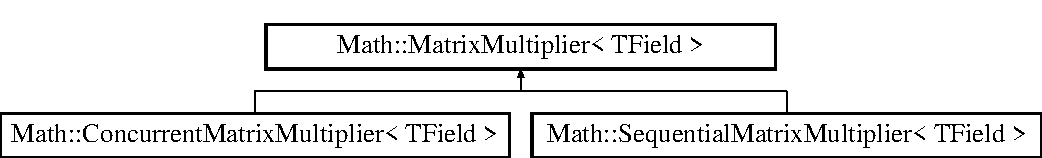
\includegraphics[height=2.000000cm]{classMath_1_1MatrixMultiplier}
\end{center}
\end{figure}
\subsection*{Public Member Functions}
\begin{DoxyCompactItemize}
\item 
\mbox{\hyperlink{classMath_1_1Matrix}{Matrix}}$<$ T\+Field $>$ \mbox{\hyperlink{classMath_1_1MatrixMultiplier_a880732c9b332798ef46e5d90f9b70625}{operator()}} (const \mbox{\hyperlink{classMath_1_1Matrix}{Matrix}}$<$ T\+Field $>$ \&A, const \mbox{\hyperlink{classMath_1_1Matrix}{Matrix}}$<$ T\+Field $>$ \&B)
\begin{DoxyCompactList}\small\item\em Called when one wants to multiply two matrices. \end{DoxyCompactList}\item 
virtual \mbox{\hyperlink{classMath_1_1MatrixMultiplier_af43501cad28dfd11f8dd73dc25edd51b}{$\sim$\+Matrix\+Multiplier}} ()
\begin{DoxyCompactList}\small\item\em Empty destructor. \end{DoxyCompactList}\end{DoxyCompactItemize}


\subsection{Detailed Description}
\subsubsection*{template$<$typename T\+Field$>$\newline
class Math\+::\+Matrix\+Multiplier$<$ T\+Field $>$}

Represents an strategy for matrix multiplication. 

Implements the function operator which, when called, checks if matrices are compatible for multiplication, and calls an abstract method, which represents the actual multiplication strategy when implemented by concrete subclasses.

\begin{DoxyAuthor}{Author}
Vitor Greati, Carlos Vieira 
\end{DoxyAuthor}
\begin{DoxyDate}{Date}
2018-\/03-\/29 
\end{DoxyDate}


\subsection{Constructor \& Destructor Documentation}
\mbox{\Hypertarget{classMath_1_1MatrixMultiplier_af43501cad28dfd11f8dd73dc25edd51b}\label{classMath_1_1MatrixMultiplier_af43501cad28dfd11f8dd73dc25edd51b}} 
\index{Math\+::\+Matrix\+Multiplier@{Math\+::\+Matrix\+Multiplier}!````~Matrix\+Multiplier@{$\sim$\+Matrix\+Multiplier}}
\index{````~Matrix\+Multiplier@{$\sim$\+Matrix\+Multiplier}!Math\+::\+Matrix\+Multiplier@{Math\+::\+Matrix\+Multiplier}}
\subsubsection{\texorpdfstring{$\sim$\+Matrix\+Multiplier()}{~MatrixMultiplier()}}
{\footnotesize\ttfamily template$<$typename T\+Field$>$ \\
virtual \mbox{\hyperlink{classMath_1_1MatrixMultiplier}{Math\+::\+Matrix\+Multiplier}}$<$ T\+Field $>$\+::$\sim$\mbox{\hyperlink{classMath_1_1MatrixMultiplier}{Matrix\+Multiplier}} (\begin{DoxyParamCaption}{ }\end{DoxyParamCaption})\hspace{0.3cm}{\ttfamily [inline]}, {\ttfamily [virtual]}}



Empty destructor. 

Allows destructing concrete classes. 

\subsection{Member Function Documentation}
\mbox{\Hypertarget{classMath_1_1MatrixMultiplier_a880732c9b332798ef46e5d90f9b70625}\label{classMath_1_1MatrixMultiplier_a880732c9b332798ef46e5d90f9b70625}} 
\index{Math\+::\+Matrix\+Multiplier@{Math\+::\+Matrix\+Multiplier}!operator()@{operator()}}
\index{operator()@{operator()}!Math\+::\+Matrix\+Multiplier@{Math\+::\+Matrix\+Multiplier}}
\subsubsection{\texorpdfstring{operator()()}{operator()()}}
{\footnotesize\ttfamily template$<$typename T\+Field$>$ \\
\mbox{\hyperlink{classMath_1_1Matrix}{Matrix}}$<$T\+Field$>$ \mbox{\hyperlink{classMath_1_1MatrixMultiplier}{Math\+::\+Matrix\+Multiplier}}$<$ T\+Field $>$\+::operator() (\begin{DoxyParamCaption}\item[{const \mbox{\hyperlink{classMath_1_1Matrix}{Matrix}}$<$ T\+Field $>$ \&}]{A,  }\item[{const \mbox{\hyperlink{classMath_1_1Matrix}{Matrix}}$<$ T\+Field $>$ \&}]{B }\end{DoxyParamCaption})\hspace{0.3cm}{\ttfamily [inline]}}



Called when one wants to multiply two matrices. 

First, perform all checks for the multiplication feasibility given the matrices, then calls a method for multiplication.


\begin{DoxyParams}{Parameters}
{\em A} & Left operator. \\
\hline
{\em B} & Right operator. \\
\hline
\end{DoxyParams}


The documentation for this class was generated from the following file\+:\begin{DoxyCompactItemize}
\item 
include/Matrix\+Multiplier.\+h\end{DoxyCompactItemize}

\hypertarget{structMatTestUtils_1_1PerfStats}{}\section{Mat\+Test\+Utils\+:\+:Perf\+Stats Struct Reference}
\label{structMatTestUtils_1_1PerfStats}\index{Mat\+Test\+Utils\+::\+Perf\+Stats@{Mat\+Test\+Utils\+::\+Perf\+Stats}}


Represent statistical estimators for the running times of the multiplication approaches.  




{\ttfamily \#include $<$Mat\+Test\+Utils.\+h$>$}

\subsection*{Public Member Functions}
\begin{DoxyCompactItemize}
\item 
\mbox{\Hypertarget{structMatTestUtils_1_1PerfStats_a263c5df4f6f542fb2f4e30d14eed2710}\label{structMatTestUtils_1_1PerfStats_a263c5df4f6f542fb2f4e30d14eed2710}} 
\mbox{\hyperlink{structMatTestUtils_1_1PerfStats_a263c5df4f6f542fb2f4e30d14eed2710}{Perf\+Stats}} ()
\begin{DoxyCompactList}\small\item\em Simple constructor. \end{DoxyCompactList}\item 
\mbox{\hyperlink{structMatTestUtils_1_1PerfStats_a3f58c1e90e5b3c9266b25ba162d34a14}{Perf\+Stats}} (const double \&\+\_\+average, const double \&\+\_\+maximum, const double \&\+\_\+minimum, const double \&\+\_\+stdeviation)
\begin{DoxyCompactList}\small\item\em Constructor taking the statistical estimators. \end{DoxyCompactList}\end{DoxyCompactItemize}
\subsection*{Public Attributes}
\begin{DoxyCompactItemize}
\item 
double \mbox{\hyperlink{structMatTestUtils_1_1PerfStats_a6b3cbd6a44fb070074555ab46918310d}{average}} = 0.\+0
\item 
double \mbox{\hyperlink{structMatTestUtils_1_1PerfStats_a584afc89a2781a9c6264bc7480439e21}{maximum}} = 0.\+0
\item 
double \mbox{\hyperlink{structMatTestUtils_1_1PerfStats_a032e057a96d030ef36355b5aac4fe596}{minimum}} = 0.\+0
\item 
double \mbox{\hyperlink{structMatTestUtils_1_1PerfStats_a103f9bae3107f94f33ff758551a1e434}{stdeviation}} = 0.\+0
\item 
std\+::vector$<$ double $>$ \mbox{\hyperlink{structMatTestUtils_1_1PerfStats_afb16d607f11552c526b636154d907a53}{running\+\_\+times}}
\end{DoxyCompactItemize}


\subsection{Detailed Description}
Represent statistical estimators for the running times of the multiplication approaches. 

\subsection{Constructor \& Destructor Documentation}
\mbox{\Hypertarget{structMatTestUtils_1_1PerfStats_a3f58c1e90e5b3c9266b25ba162d34a14}\label{structMatTestUtils_1_1PerfStats_a3f58c1e90e5b3c9266b25ba162d34a14}} 
\index{Mat\+Test\+Utils\+::\+Perf\+Stats@{Mat\+Test\+Utils\+::\+Perf\+Stats}!Perf\+Stats@{Perf\+Stats}}
\index{Perf\+Stats@{Perf\+Stats}!Mat\+Test\+Utils\+::\+Perf\+Stats@{Mat\+Test\+Utils\+::\+Perf\+Stats}}
\subsubsection{\texorpdfstring{Perf\+Stats()}{PerfStats()}}
{\footnotesize\ttfamily Mat\+Test\+Utils\+::\+Perf\+Stats\+::\+Perf\+Stats (\begin{DoxyParamCaption}\item[{const double \&}]{\+\_\+average,  }\item[{const double \&}]{\+\_\+maximum,  }\item[{const double \&}]{\+\_\+minimum,  }\item[{const double \&}]{\+\_\+stdeviation }\end{DoxyParamCaption})\hspace{0.3cm}{\ttfamily [inline]}}



Constructor taking the statistical estimators. 


\begin{DoxyParams}{Parameters}
{\em \+\_\+average} & \\
\hline
{\em \+\_\+maximum} & \\
\hline
{\em \+\_\+minimum} & \\
\hline
{\em \+\_\+stdeviation} & \\
\hline
\end{DoxyParams}


\subsection{Member Data Documentation}
\mbox{\Hypertarget{structMatTestUtils_1_1PerfStats_a6b3cbd6a44fb070074555ab46918310d}\label{structMatTestUtils_1_1PerfStats_a6b3cbd6a44fb070074555ab46918310d}} 
\index{Mat\+Test\+Utils\+::\+Perf\+Stats@{Mat\+Test\+Utils\+::\+Perf\+Stats}!average@{average}}
\index{average@{average}!Mat\+Test\+Utils\+::\+Perf\+Stats@{Mat\+Test\+Utils\+::\+Perf\+Stats}}
\subsubsection{\texorpdfstring{average}{average}}
{\footnotesize\ttfamily double Mat\+Test\+Utils\+::\+Perf\+Stats\+::average = 0.\+0}

Average running time. \mbox{\Hypertarget{structMatTestUtils_1_1PerfStats_a584afc89a2781a9c6264bc7480439e21}\label{structMatTestUtils_1_1PerfStats_a584afc89a2781a9c6264bc7480439e21}} 
\index{Mat\+Test\+Utils\+::\+Perf\+Stats@{Mat\+Test\+Utils\+::\+Perf\+Stats}!maximum@{maximum}}
\index{maximum@{maximum}!Mat\+Test\+Utils\+::\+Perf\+Stats@{Mat\+Test\+Utils\+::\+Perf\+Stats}}
\subsubsection{\texorpdfstring{maximum}{maximum}}
{\footnotesize\ttfamily double Mat\+Test\+Utils\+::\+Perf\+Stats\+::maximum = 0.\+0}

Maximum running time. \mbox{\Hypertarget{structMatTestUtils_1_1PerfStats_a032e057a96d030ef36355b5aac4fe596}\label{structMatTestUtils_1_1PerfStats_a032e057a96d030ef36355b5aac4fe596}} 
\index{Mat\+Test\+Utils\+::\+Perf\+Stats@{Mat\+Test\+Utils\+::\+Perf\+Stats}!minimum@{minimum}}
\index{minimum@{minimum}!Mat\+Test\+Utils\+::\+Perf\+Stats@{Mat\+Test\+Utils\+::\+Perf\+Stats}}
\subsubsection{\texorpdfstring{minimum}{minimum}}
{\footnotesize\ttfamily double Mat\+Test\+Utils\+::\+Perf\+Stats\+::minimum = 0.\+0}

Minium running time. \mbox{\Hypertarget{structMatTestUtils_1_1PerfStats_afb16d607f11552c526b636154d907a53}\label{structMatTestUtils_1_1PerfStats_afb16d607f11552c526b636154d907a53}} 
\index{Mat\+Test\+Utils\+::\+Perf\+Stats@{Mat\+Test\+Utils\+::\+Perf\+Stats}!running\+\_\+times@{running\+\_\+times}}
\index{running\+\_\+times@{running\+\_\+times}!Mat\+Test\+Utils\+::\+Perf\+Stats@{Mat\+Test\+Utils\+::\+Perf\+Stats}}
\subsubsection{\texorpdfstring{running\+\_\+times}{running\_times}}
{\footnotesize\ttfamily std\+::vector$<$double$>$ Mat\+Test\+Utils\+::\+Perf\+Stats\+::running\+\_\+times}

Sequence of running times registered in the test. \mbox{\Hypertarget{structMatTestUtils_1_1PerfStats_a103f9bae3107f94f33ff758551a1e434}\label{structMatTestUtils_1_1PerfStats_a103f9bae3107f94f33ff758551a1e434}} 
\index{Mat\+Test\+Utils\+::\+Perf\+Stats@{Mat\+Test\+Utils\+::\+Perf\+Stats}!stdeviation@{stdeviation}}
\index{stdeviation@{stdeviation}!Mat\+Test\+Utils\+::\+Perf\+Stats@{Mat\+Test\+Utils\+::\+Perf\+Stats}}
\subsubsection{\texorpdfstring{stdeviation}{stdeviation}}
{\footnotesize\ttfamily double Mat\+Test\+Utils\+::\+Perf\+Stats\+::stdeviation = 0.\+0}

Standard deviation regarding the running times. 

The documentation for this struct was generated from the following file\+:\begin{DoxyCompactItemize}
\item 
include/Mat\+Test\+Utils.\+h\end{DoxyCompactItemize}

\hypertarget{classMath_1_1SequentialMatrixMultiplier}{}\section{Math\+:\+:Sequential\+Matrix\+Multiplier$<$ T\+Field $>$ Class Template Reference}
\label{classMath_1_1SequentialMatrixMultiplier}\index{Math\+::\+Sequential\+Matrix\+Multiplier$<$ T\+Field $>$@{Math\+::\+Sequential\+Matrix\+Multiplier$<$ T\+Field $>$}}


Provides a method for multiplying matrices based on the mathematical definition sequentially (single-\/thread).  




{\ttfamily \#include $<$Sequential\+Matrix\+Multiplier.\+h$>$}

Inheritance diagram for Math\+:\+:Sequential\+Matrix\+Multiplier$<$ T\+Field $>$\+:\begin{figure}[H]
\begin{center}
\leavevmode
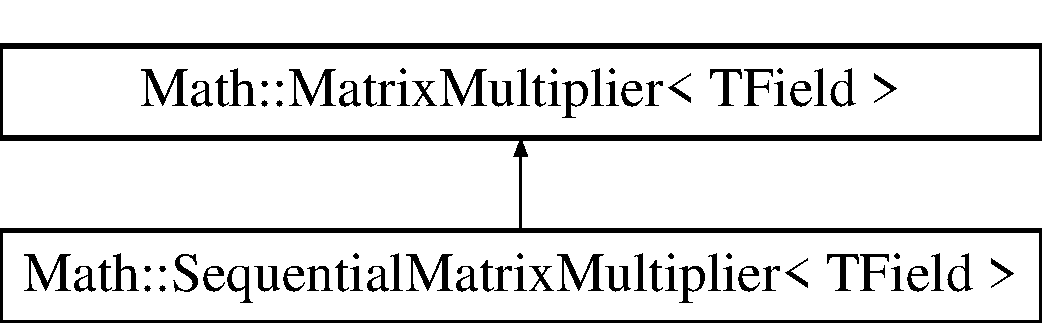
\includegraphics[height=2.000000cm]{classMath_1_1SequentialMatrixMultiplier}
\end{center}
\end{figure}
\subsection*{Public Member Functions}
\begin{DoxyCompactItemize}
\item 
void \mbox{\hyperlink{classMath_1_1SequentialMatrixMultiplier_ac50584976bf8efe3a0a755048c427753}{multiply}} (const \mbox{\hyperlink{classMath_1_1Matrix}{Matrix}}$<$ T\+Field $>$ \&A, const \mbox{\hyperlink{classMath_1_1Matrix}{Matrix}}$<$ T\+Field $>$ \&B, \mbox{\hyperlink{classMath_1_1Matrix}{Matrix}}$<$ T\+Field $>$ \&prod)
\begin{DoxyCompactList}\small\item\em Computes the product of two matrices using the algorithm from the mathematical definition, using a single thread. \end{DoxyCompactList}\end{DoxyCompactItemize}


\subsection{Detailed Description}
\subsubsection*{template$<$typename T\+Field$>$\newline
class Math\+::\+Sequential\+Matrix\+Multiplier$<$ T\+Field $>$}

Provides a method for multiplying matrices based on the mathematical definition sequentially (single-\/thread). 

\begin{DoxyAuthor}{Author}
Vitor Greati, Carlos Vieira 
\end{DoxyAuthor}
\begin{DoxyDate}{Date}
2018-\/03-\/28 
\end{DoxyDate}


\subsection{Member Function Documentation}
\mbox{\Hypertarget{classMath_1_1SequentialMatrixMultiplier_ac50584976bf8efe3a0a755048c427753}\label{classMath_1_1SequentialMatrixMultiplier_ac50584976bf8efe3a0a755048c427753}} 
\index{Math\+::\+Sequential\+Matrix\+Multiplier@{Math\+::\+Sequential\+Matrix\+Multiplier}!multiply@{multiply}}
\index{multiply@{multiply}!Math\+::\+Sequential\+Matrix\+Multiplier@{Math\+::\+Sequential\+Matrix\+Multiplier}}
\subsubsection{\texorpdfstring{multiply()}{multiply()}}
{\footnotesize\ttfamily template$<$typename T\+Field $>$ \\
void \mbox{\hyperlink{classMath_1_1SequentialMatrixMultiplier}{Math\+::\+Sequential\+Matrix\+Multiplier}}$<$ T\+Field $>$\+::multiply (\begin{DoxyParamCaption}\item[{const \mbox{\hyperlink{classMath_1_1Matrix}{Matrix}}$<$ T\+Field $>$ \&}]{A,  }\item[{const \mbox{\hyperlink{classMath_1_1Matrix}{Matrix}}$<$ T\+Field $>$ \&}]{B,  }\item[{\mbox{\hyperlink{classMath_1_1Matrix}{Matrix}}$<$ T\+Field $>$ \&}]{prod }\end{DoxyParamCaption})\hspace{0.3cm}{\ttfamily [inline]}, {\ttfamily [virtual]}}



Computes the product of two matrices using the algorithm from the mathematical definition, using a single thread. 


\begin{DoxyParams}{Parameters}
{\em A} & Left operand. \\
\hline
{\em B} & Right operand. \\
\hline
{\em prod} & Product matrix. \\
\hline
\end{DoxyParams}


Implements \mbox{\hyperlink{classMath_1_1MatrixMultiplier}{Math\+::\+Matrix\+Multiplier$<$ T\+Field $>$}}.



The documentation for this class was generated from the following file\+:\begin{DoxyCompactItemize}
\item 
include/Sequential\+Matrix\+Multiplier.\+h\end{DoxyCompactItemize}

%--- End generated contents ---

% Index
\backmatter
\newpage
\phantomsection
\clearemptydoublepage
\addcontentsline{toc}{chapter}{Index}
\printindex

\end{document}
